\documentclass[class=report, float=false, crop=false]{standalone}
%  \usepackage[subpreambles=true]{standalone}

\usepackage{pgf, tikz}
\usetikzlibrary{shapes.misc}
\usetikzlibrary{decorations.pathreplacing}

\tikzset{cross/.style={cross out, draw=black, minimum size=2*(#1-\pgflinewidth), inner sep=0pt, outer sep=0pt},
%default radius will be 1pt. 
cross/.default={0.25pt},
    point/.style={
    thick,
    draw=black,
    cross out,
    inner sep=0pt,
    minimum width=4pt,
    minimum height=4pt,
    },
}

\graphicspath{{figures/figs/}}

% \begin{cbunit}

\begin{document}

\chapter{Results and discussion}
\label{chap:results}

\section{Preliminary results}

Preliminary simulations were performed with only 64 particles, first to ensure that the our models and methods gave realistic results, then to determine what phenomena were different with ellipsoids than with spheres. Simulations performed with this few particles have the advantage to quickly give results to analyse, however finite-size effects are not negligible and can affect the jamming transition (see part \ref{finite-size_effects}).

\subsection{Rheological transition}

\begin{figure}[h!]
\centering
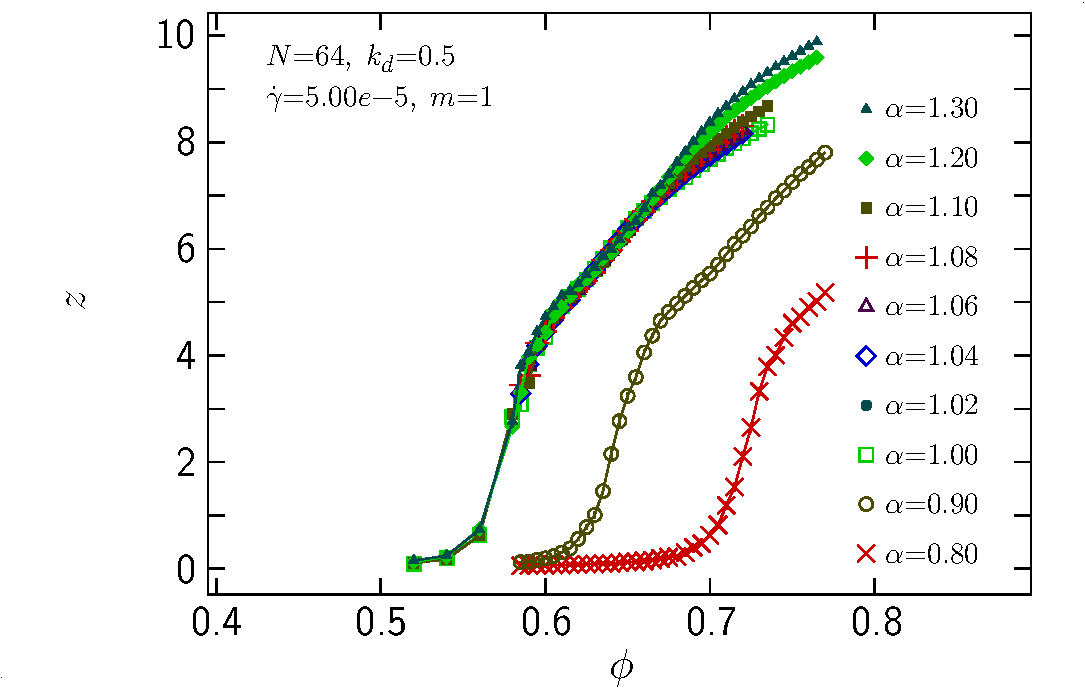
\includegraphics[width=0.6\textwidth]{figures/figs/z_phi_0064_KDk500_Ml100_GDg500}
\caption{Average contact number per particle as a function of the packing fraction for aspect ratios $0.8\le\alpha\le1.3$. $N=64,~ k_d=0.5,~ \dot{\gamma}=5e-5,~ m=1$.}
\label{z_phi_0064_KDk500_Ml100_GDg500}
\end{figure}

\begin{figure}[h!]
\centering
    \begin{subfigure}[t]{0.32\textwidth}
        \centering
        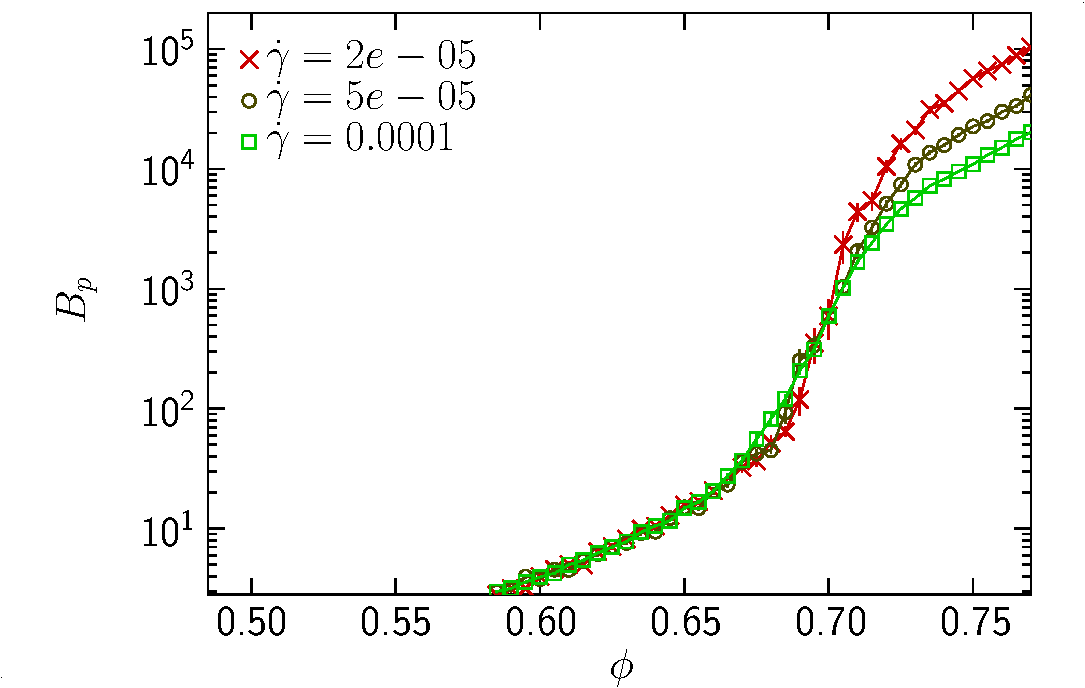
\includegraphics[width=\textwidth]{figures/figs/bp_0064_KDk500_Ml100_EL080}
        \caption{$\alpha=0.8$, $\phi_C\sim0.72$}
        \label{bp_0064_KDk500_Ml100_EL080}
    \end{subfigure}
    \hfill
    \begin{subfigure}[t]{0.32\textwidth}
        \centering
        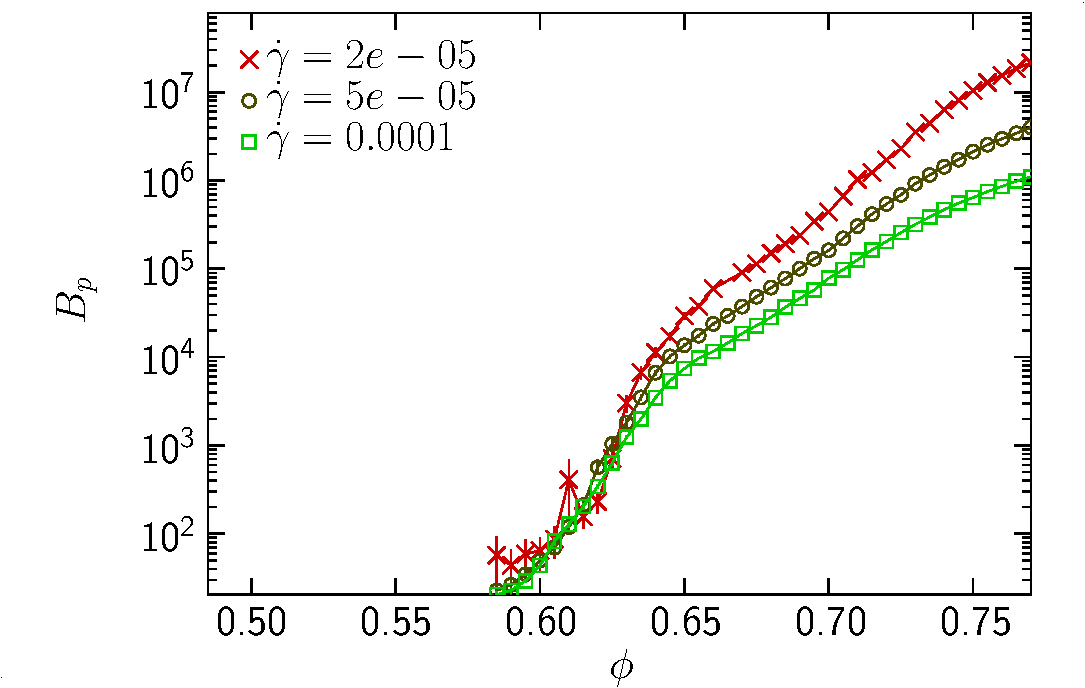
\includegraphics[width=\textwidth]{figures/figs/bp_0064_KDk500_Ml100_EL090}
        \caption{$\alpha=0.9$, $\phi_C\sim0.63$}
        \label{bp_0064_KDk500_Ml100_EL090}
    \end{subfigure}
    \hfill
    \begin{subfigure}[t]{0.32\textwidth}
        \centering
        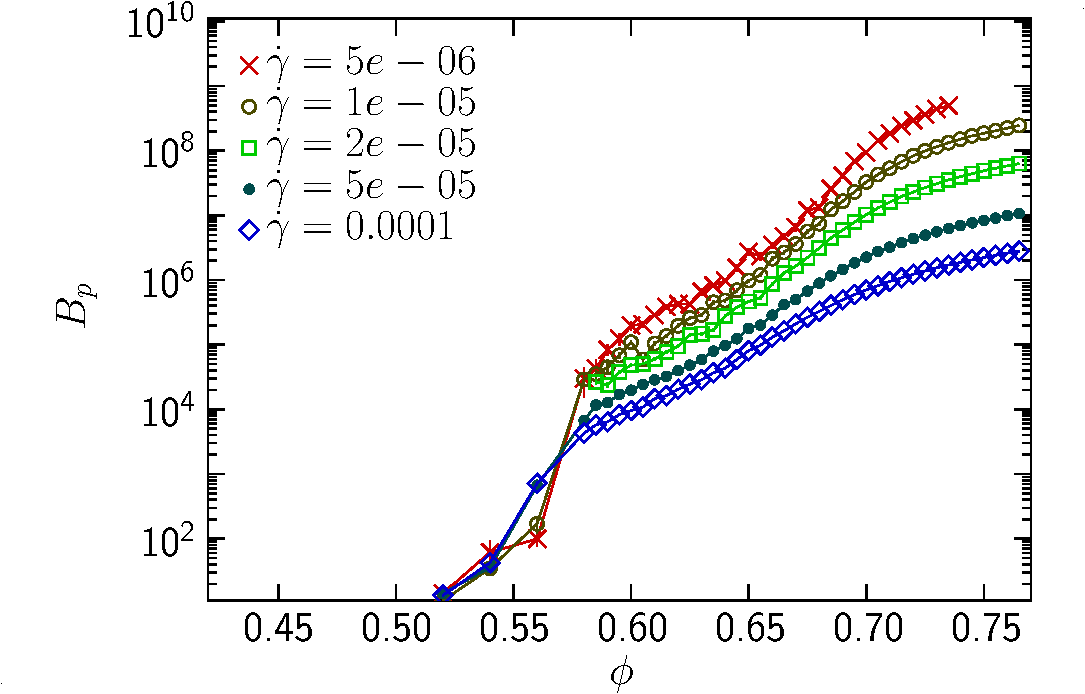
\includegraphics[width=\textwidth]{figures/figs/bp_0064_KDk500_Ml100_EL130}
        \caption{$\alpha=1.3$, $\phi_C\sim0.57$}
        \label{bp_0064_KDk500_Ml100_EL130}
    \end{subfigure}
    
    \vspace{0pt}
    \begin{subfigure}[t]{0.32\textwidth}
        \centering
        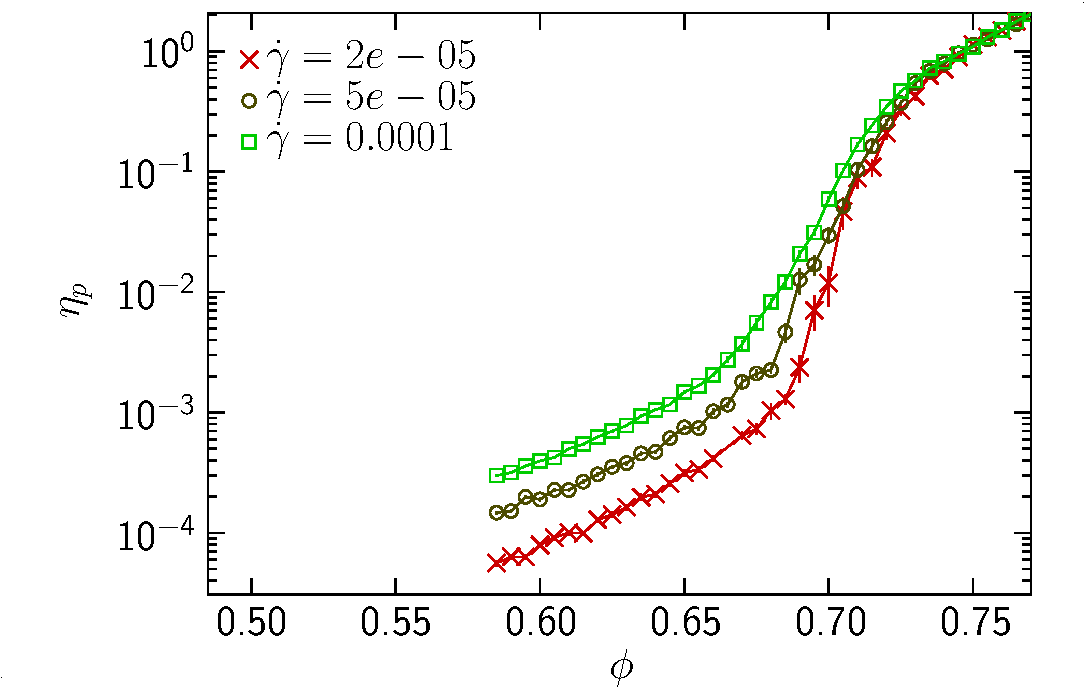
\includegraphics[width=\textwidth]{figures/figs/etap_0064_KDk500_Ml100_EL080}
        \caption{$\alpha=0.8$, $\phi_C\sim0.72$}
        \label{etap_0064_KDk500_Ml100_EL080}
    \end{subfigure}
    \hfill
    \begin{subfigure}[t]{0.32\textwidth}
        \centering
        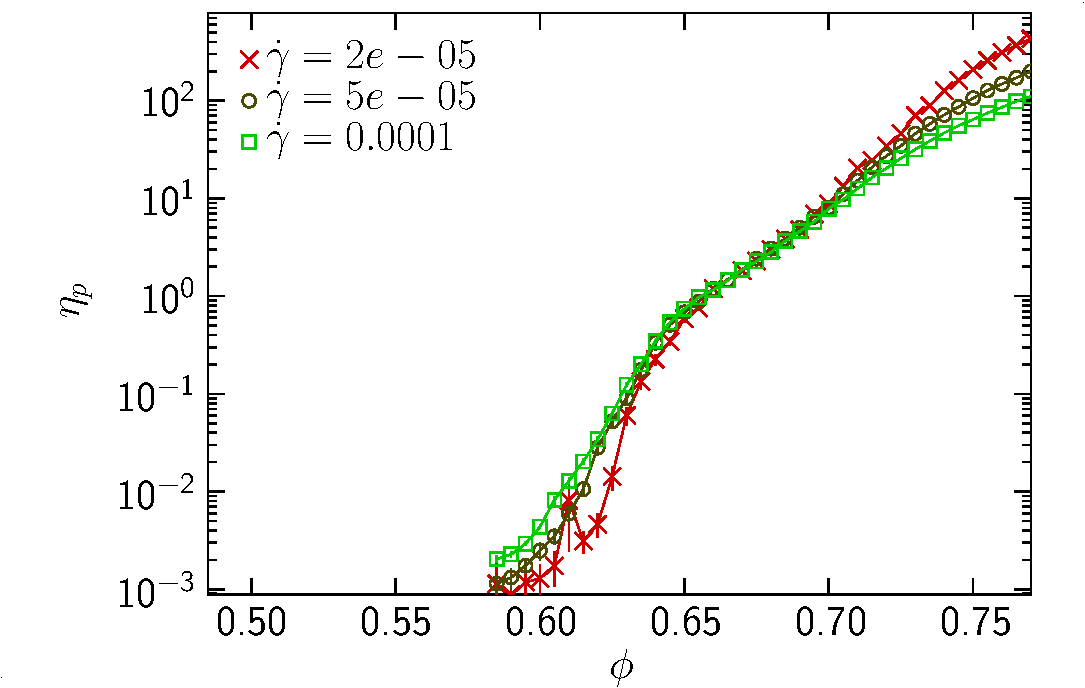
\includegraphics[width=\textwidth]{figures/figs/etap_0064_KDk500_Ml100_EL090}
        \caption{$\alpha=0.9$, $\phi_C\sim0.63$}
        \label{etap_0064_KDk500_Ml100_EL090}
    \end{subfigure}
    \hfill
    \begin{subfigure}[t]{0.32\textwidth}
        \centering
        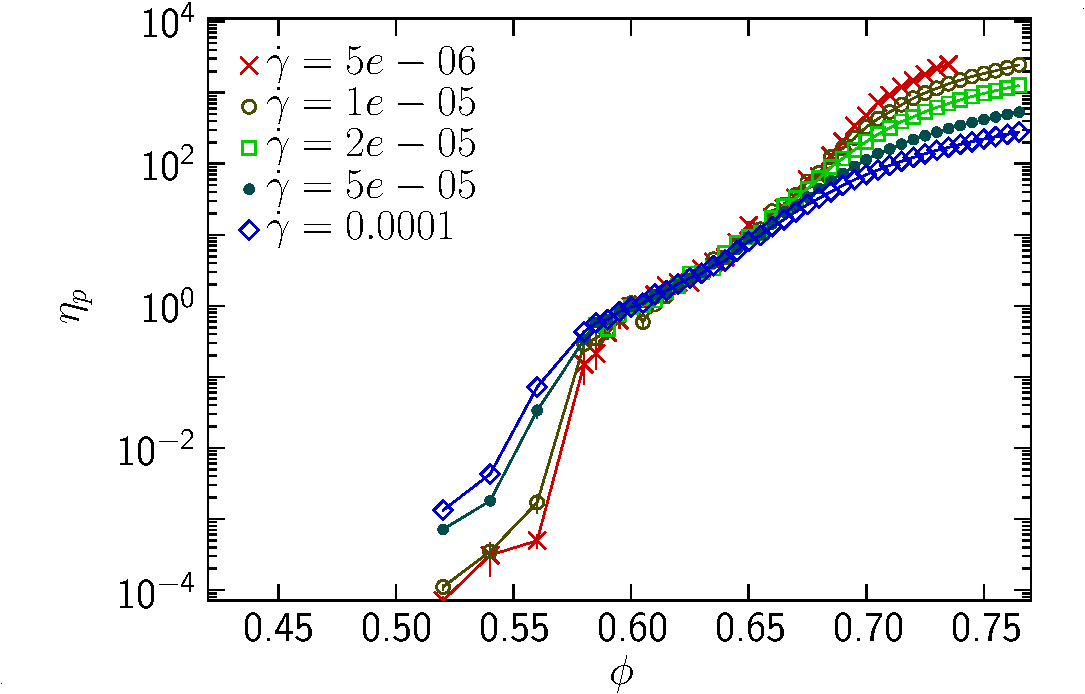
\includegraphics[width=\textwidth]{figures/figs/etap_0064_KDk500_Ml100_EL130}
        \caption{$\alpha=1.3$, $\phi_C\sim0.57$}
        \label{etap_0064_KDk500_Ml100_EL130}
    \end{subfigure}
\caption{Bagnoldian (figures \ref{bp_0064_KDk500_Ml100_EL080}, \ref{bp_0064_KDk500_Ml100_EL090} and \ref{bp_0064_KDk500_Ml100_EL130}) and Newtonian (figures \ref{etap_0064_KDk500_Ml100_EL080}, \ref{etap_0064_KDk500_Ml100_EL090} and \ref{etap_0064_KDk500_Ml100_EL130}) transport coefficients associated to pressure. $N=64,~ k_d=0.5,~ m=1$. We denote $\phi_C$ the transition packing fraction.}
\label{rheo_0064}
\end{figure}

We observe in figure \ref{z_phi_0064_KDk500_Ml100_GDg500} a sharp increase in the average contact number per particle upon increasing the packing fraction. According to the development of part \ref{rheology}, this increase is the sign of a transition from Bagnoldian rheology to Newtonian rheology. We confirm this by determining the Bagnoldian and Newtonian transport coefficients associated to pressure as functions of the packing fraction, and verifying the transitions from a regime to the other occurs at the same packing fractions as the increase of contact number (figure \ref{rheo_0064}).\\

We also observe that the Newtonian transport coefficients become $\dot{\gamma}$-dependent for high enough packing fractions, we will see further that this is due to a deviation from the hard-core limit near the jamming transition.\\

Moreover, we can notice that for $1\le\alpha<1.3$ (sphere and prolate spheroids) the transition from the Bagnoldian to the Newtonian regime occurs approximately at the same packing fraction, while for $\alpha=0.8,0.9$ (oblate spheroids) the transition packing fraction $\phi_C$ varies with the aspect ratio and is higher than the value obtained for the former particles.

\subsection{Critical behaviour}

\subsubsection{Effectiveness of scaling}

\subsubsection{Jamming density and critical exponent}

\subsection{Orientation correlation}

\subsection{Rotation velocity}

\section{Dominance of elastic pressure}

**** SHOW THAT THE MAIN CONTRIBUTION TO PRESSURE IS THE ELASTIC PRESSURE ****

% \addcontentsline{toc}{section}{References}
\bibliographystyle{unsrtnat}
\bibliography{references/biblio}
{\renewcommand{\bibname}{References}\bibliography{references/biblio}}

\end{document}

% \end{cbunit}